%===============================================================================
% (c) Dominik Harmim


\chapter{Introduction}

Bugs are an integral part of computer programs ever since the inception
of the programming discipline. Unfortunately, they are often hidden
in unexpected places, and they can lead to unexpected behaviour which
may cause significant damage. Nowadays there are many possible
ways of catching bugs in the development process. Dynamic analysis
tools or tools for automated testing are often used. These methods
are satisfactory in many cases. Nevertheless, they can still leave
too many bugs undetected, because they are able to analyse only
certain program flows, dependent on its input data. An alternative
solution is a~\emph{static analysis}. Of course, it has some shortages
as well. The big issue is \emph{scalability} on extensive codebases and
considerable high rate of incorrectly reported errors (so-called
\emph{false positives}, also called \emph{false alarms}).

Not long ago, Facebook introduced \emph{Facebook Infer}\,--\,a~tool for
creating \emph{highly scalable} \emph{compositional}, \emph{incremental},
and \emph{interprocedural} static analysers. Facebook Infer is a~live tool
and it is still under the development. Anyway, it is in everyday use in
Facebook itself, Spotify, Uber, Mozilla, WhatsApp and other well-known
companies. Currently, Facebook Infer provides several analysers implemented
as modules in the whole framework. These analysers check for various types
of bugs, e.g., buffer overflows, thread-safety, null-dereferencing, or
memory leaks. Facebook Infer also aims to create a~framework for building
new analysers quickly and easily. The current version of Facebook Infer still
misses better support for \emph{concurrency} bugs. While it provides a~fairly
advanced \emph{data race} analyser, it is limited to Java programs only and
fails for C~programs, which require more through manipulation with locks.

In \emph{concurrent programs}, there are often \emph{atomicity requirements}
for execution of specific sequences of instructions. Violating these
requirements may cause many kinds of problems, such as unexpected
behaviour, exceptions, segmentation faults, or other failures.
\emph{Atomicity violations} are usually not verified by compilers,
unlike syntactic or some sorts of semantic rules. Atomicity requirements,
in most cases, are not even documented. It means that typically only
programmers must take care of following these requirements. In general,
it is very difficult to avoid errors in \emph{atomicity-dependent
programs}, especially in large projects, and even harder and time-consuming
is finding and fixing these errors.

In this thesis, there is described proposal, implementation, and experimental
verification and evaluation of \emph{Atomer}\,---\,static analyser for
finding atomicity violations\,---\,which is implemented as an extension for
Facebook Infer. In particular, the concentration is put on an
\emph{atomic execution of sequences of function calls}, which is often
required, e.g., when using certain library calls. The implementation targets
to C/C++ programs that use \emph{PThreads} locks.

The development of \emph{Atomer} has been discussed with developers of
Facebook Infer, and it is a~part of the H2020 ECSEL project Aquas. Parts
of this paper are taken over~\cite{excel2019FBInfer}, which I~wrote
together with Vladimír Marcin and Ondřej Pavela. In~\cite{excel2019FBInfer},
there was presented preliminary results of my thesis.

The rest of the paper is organised as follows. In
Chapter~\ref{chap:preliminaries}, there are described all the topics
which are necessary to understand before reading the rest of the paper. In
particular, Section~\ref{sec:staticAnalysisAI} deals with
a~\emph{static analysis} based on \emph{abstract interpretation}.
Facebook Infer, which uses abstract interpretation, is described in
Section~\ref{sec:fbinfer}. And in Section~\ref{sec:contracts}, there is
described the concept of \emph{contracts for concurrency}. Proposal of a~static
analyser for detection \emph{atomicity violations}, based on this concept, is
described in Chapter~\ref{chap:proposal}. Its implementation is in
Chapter~\ref{chap:implementation} and experimental results are presented
in Chapter~\ref{chap:experiments}. Finally, Chapter~\ref{chap:conclusion}
concludes the paper. Appendix~\ref{chap:memoryMedia} lists contents
of attached memory media and Appendix~\ref{chap:manual} serves as an
installation and user manual.



\chapter{Preliminaries}
\label{chap:preliminaries}

This chapter explains the theoretical background on which stands the
thesis. It also explains and describes the existing tools used in the
thesis. Lastly, the chapter deals with existing solutions and principles
which this thesis got inspired by.

The aim of this thesis is to propose a~\emph{static analyser} and implement
it in \emph{Facebook Infer}. So, in Section~\ref{sec:staticAnalysisAI},
there is a~brief explanation of a~\emph{static analysis} itself, and then an
explanation of \emph{abstract interpretation} that is used in Facebook Infer.
Facebook Infer, its principles and features illustrate
Section~\ref{sec:fbinfer}. The proposal of a~solution is based on the
concept of \emph{contracts for concurrency}, which is discussed and defined
in Section~\ref{sec:contracts}.


\section{Static Analysis by Abstract Interpretation}
\label{sec:staticAnalysisAI}

According to~\cite{staticAnalysisMoller}, a~\emph{static analysis} of
programs is reasoning about the behaviour of computer programs without
actually executing them. It has been used since the 1970s for optimising
compilers for generating effective code. More recently, it has proven
valuable also for automatic error detection, verification tools and it
is used in other tools that can help programmers. Intuitively,
a~static program analyser is a~program that reasons about the behaviour
of other programs, in other words, a~static program analyser checks if the
\emph{program semantics} of a~given program fulfils the given
\emph{specification}, as illustrates Figure~\ref{fig:staticAnalysis}
\cite{AIBasedFormalMethodsCousot}. Nowadays, a~static analysis is one of
the fundamental concepts of \emph{formal verification}. It aims to
automatically answer questions about a~given program, such as
e.g.~\cite{staticAnalysisMoller}:
\begin{itemize}
    \item
        \textbf{Are certain operations executed \emph{atomically}?}

    \item
        Does the program terminate on every input?

    \item
        Can the program \emph{deadlock}?

    \item
        Does there exist an input that leads to a~\emph{null-pointer
        dereference}, a~\emph{division-by-zero}, or an \emph{arithmetic
        overflow}?

    \item
        Are all variable initialised before they are used?

    \item
        Are arrays always accessed within their bound?

    \item
        Does the program contain \emph{dead code}?

    \item
        Are all resources correctly released after their last
        use?
\end{itemize}

\begin{figure}[htb]
    \centering
    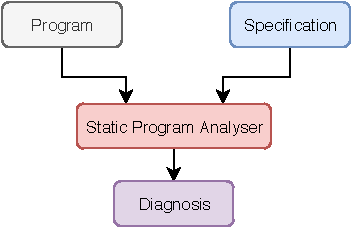
\includegraphics[width=.4 \linewidth]{static_analysis.pdf}
    \caption{
        Static program analysis (inspired
        by~\cite{AIBasedFormalMethodsCousot})
    }
    \label{fig:staticAnalysis}
\end{figure}

It is well-known that testing, i.e., executing programs
with some input data and examining the output, may expose errors, but it
can not prove their absence. (It was also famously stated by Edsger W.
Dijkstra: \uv{\textit{Program testing can be used to show the presence of bugs,
but never to show their absence!}}.) However, a~static program analysis
can prove their absence\,---\,with some \emph{approximation}\,---\,it can
check \emph{all possible executions} of the programs and provide guarantees
about their properties. Another advantage of static analysis is that the
analysis can be performed during the development process, so the program
does not have to be executable yet and it already can be analysed.
The significant issue is how to ensure high precision and
\emph{scalability} to be useful in practice. The biggest disadvantage is
that static analysis can produce many \emph{false alarms}\footnote{
\emph{False alarms}\,--\,incorrectly reported an error. Also called
\emph{false positives}.}, but it is often
resolved by accepting \emph{unsoundness}\footnote{\emph{Soundness}\,--\,if
a~verification method claims that a~system is correct according to a~given
specification, it is truly correct.~\cite{favStaticAnalysis}}.

Various forms of a~static analysis of programs have been invented, for
instance~\cite{favStaticAnalysis}: bug pattern searching, data-flow
analysis, constraint-based analysis, type analysis, symbolic execution. And
one of the essential concept\,---\,\emph{abstract interpretation}\,---\,is
detailed in Section~\ref{sec:AI}.

There exist numerous tools for static analysis (often proprietary and
difficult to openly evaluate or extend), e.g.: Coverity, Klockwork, CodeSonar,
Loopus, phpstan, or \emph{Facebook Infer} (described in
Section~\ref{sec:fbinfer}).


\subsection{Abstract Interpretation}
\label{sec:AI}

This section explains and defines the basics of \emph{abstract interpretation}.
The description is based on~\cite{AIBasedFormalMethodsCousot},
\cite{AILatticeModelCousot}, \cite{AIInNutshellCousot}, \cite{AICousotWeb},
\cite{favAI}, \cite{projectPracticeMarcin2018}, \cite{wideningNarrowingCousot},
\cite{programAnalysisNielson}, \cite{staticAnalysisMoller},
\cite{favLatticesAndFixpoints}. In these bibliographies, there also can be
found more detailed, more formal, and a~more theoretical explanation.

The abstract interpretation was introduced and formalised by a~French
computer scientist Patrick Cousot and his wife Radhia Cousot in the year
1977 at POPL\footnote{POPL\,--\,symposium on Principles of Programming
Languages.}~\cite{AILatticeModelCousot}. It is a~generic \emph{framework}
for static analyses. It is possible to create particular analyses by
providing specific components (described later) to the framework. The
analysis is guaranteed to be \emph{sound} if certain properties of the
components are met.~\cite{favAI}, \cite{projectPracticeMarcin2018}

In general, in the set theory, which is independent on an application
setting, abstract interpretation is considered theory for
\emph{approximating} sets and set operations. A~more restricted formulation
of abstract interpretation is to interpret it as a~theory of approximation
of the behaviour of the \emph{formal semantics} of programs. Those
behaviours may be characterised by \emph{fixpoints} (defined below), that is
why a~primary part of the theory provides efficient techniques for
\emph{fixpoint approximation}~\cite{programAnalysisNielson}.
So, for a~standard semantics, abstract interpretation is used to derive
the approximate abstract semantics over an \emph{abstract domain} (defined
below), in order to check a~given \emph{program specification} using
analysation of the abstract semantics.~\cite{AIBasedFormalMethodsCousot}

Patrick Cousot intuitively and informally illustrates abstract
interpretation in~\cite{AIInNutshellCousot} as follows.
Figure~\ref{fig:ai1} shows the \emph{concrete semantics} of a~program
by a~set of curves, which represents the set of all possible executions
of the program in all possible execution environments. Each curve shows
the evolution of the vector~$ x(t) $~of input values, state, and
output values of the program as a~function of the time~$ t $.
\emph{Forbidden zones} on this figure represent a~set of erroneous states
of the program execution. Proving, that the intersection of the concrete
semantics of the program with the forbidden zone is empty, is undecidable
because the program concrete semantics is not computable. As demonstrates
Figure~\ref{fig:ai2}, abstract interpretation deals with an
\emph{abstract semantics}, i.e., the \emph{superset} of the concrete
program semantics. The abstract semantics includes all possible executions.
That implies that if the abstract semantics is safe (i.e. does not
intersect the forbidden zone), concrete semantics is safe as well. However,
the \emph{over-approximation} of the possible program executions causes
that inexisting program executions are considered, that may lead to
\emph{false alarms}. It is the case when the abstract semantics
intersects the forbidden zone, whereas the concrete semantics does not
intersect it.

\begin{figure}[htb]
     \centering

     \begin{subfigure}[htb]{.45 \linewidth}
         \centering
         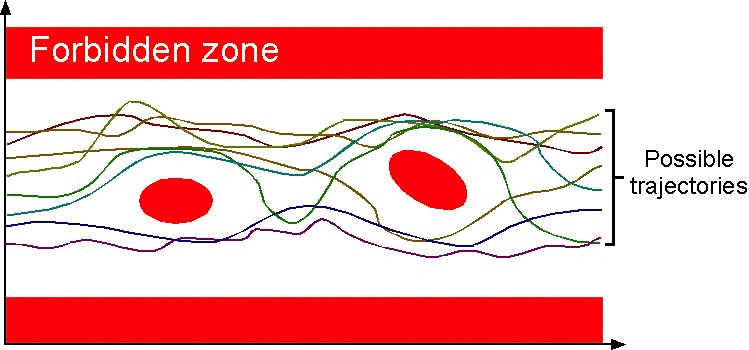
\includegraphics[width=1 \linewidth]{ai_1.png}
         \caption{
            \emph{Concrete semantics} of programs with
            \emph{forbidden zones}
        }
         \label{fig:ai1}
     \end{subfigure}
%
     \hfill
%
     \begin{subfigure}[htb]{.45\linewidth}
         \centering
         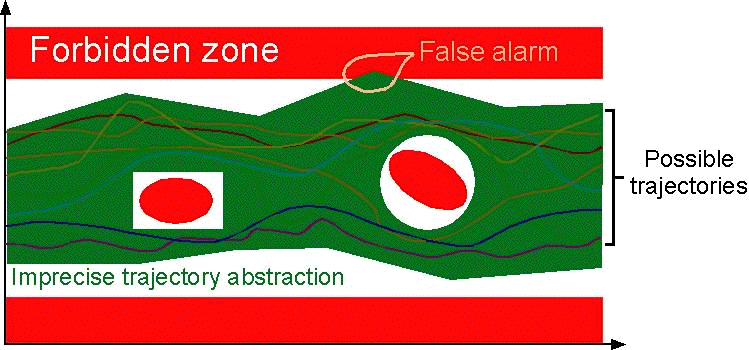
\includegraphics[width=1 \linewidth]{ai_2.png}
         \caption{
            \emph{Abstract semantics} of programs with imprecise
            trajectory abstraction
        }
         \label{fig:ai2}
     \end{subfigure}
%
    \caption{
        \emph{Abstract interpretation} demonstration~\cite{AIInNutshellCousot}.
        Horizontal axes: the time~$ t $. Vertical axes: the
        vector~$ x(t) $~of the input values of programs
    }
\end{figure}

\subsubsection*{Components of Abstract Interpretation}

In accordance with~\cite{favAI}, \cite{projectPracticeMarcin2018},
basic components of abstract interpretation are as follows:
\begin{itemize}
    \item \textbf{Abstract Domain}~\cite{AICousotWeb}
        \begin{itemize}
            \item
                An abstraction of the \emph{concrete semantics} in the form
                of \emph{abstract properties}\footnote{\emph{Abstract
                properties} approximating \emph{concrete properties
                behaviours}.} and \emph{abstract
                operations}\footnote{\emph{Abstract operations} include
                abstractions of the \emph{concrete approximation}, an
                approximation of the \emph{concrete fixpoint transform
                function}, etc.}.~\cite{AIBasedFormalMethodsCousot}

            \item
                Sets of program states at certain locations are represented
                using \emph{abstract states}.
        \end{itemize}

    \item \textbf{Abstract Transformers}
        \begin{itemize}
            \item
                There is a~\emph{transform function} for each program
                operation (instruction) that represents the impact
                of the operation executed on an abstract state.
        \end{itemize}

    \item \textbf{Join Operator}~$ \circ $
        \begin{itemize}
            \item
                Joins abstract states from individual program branches into
                a~single one.
        \end{itemize}

    \item
        \textbf{Widening
        Operator~$ \triangledown $}~\cite{programAnalysisNielson},
        \cite{wideningNarrowingCousot}, \cite{favAI}
        \begin{itemize}
            \item
                Enforces termination of the abstract interpretation.

            \item
                It is used to approximate the \emph{least fixed points}
                (it is performed on a~sequence of abstract states at
                a~certain location).

            \item
                The later in the analysis is this operator used, the more
                accurate is the result (but the analysis takes more time).
        \end{itemize}

    \item
        \textbf{Narrowing
        Operator~$ \vartriangle $}~\cite{programAnalysisNielson},
        \cite{wideningNarrowingCousot}, \cite{favAI}
        \begin{itemize}
            \item
                Encapsulates a~termination criterion.

            \item
                Using this operator, the approximation can be refined, i.e.,
                it may be used to refine the result of widening.

            \item
                This operator is used when a~\emph{fixpoint} is
                approximated using widening.
        \end{itemize}
\end{itemize}

\subsubsection*{Fixpoints and Fixpoint Approximation}

In~\cite{favLatticesAndFixpoints}, there is a~\emph{fixpoint} defined as:
\begin{itemize}
    \item
        let $ (A, \leq_A) $ be a~\emph{lattice}~\cite{favLatticesAndFixpoints},

    \item
        an element $ a \in A $ is a~\textbf{fixpoint} of a~function
        $ f : A \rightarrow A $ if and only if $ \boldsymbol{f(a) = a} $.
\end{itemize}
Computation of the \emph{most precise abstract fixpoint} is not generally
guaranteed to terminate in certain cases, such as loops. The solution is
to approximate the fixpoint using \emph{widening} (over-approximation of
a~fixpoint) and \emph{narrowing} (improves an approximation of
a~fixpoint)~\cite{favAI}, \cite{projectPracticeMarcin2018}.
Most program properties can be represented as fixpoints. This reduces program
analysis to the fixpoint approximation~\cite{AICousotWeb}. Further
information about fixpoint approximation can be found
in~\cite{programAnalysisNielson}, \cite{wideningNarrowingCousot}.

\subsubsection*{Formal Definition of Abstract Interpretation}

According to~\cite{AILatticeModelCousot}, \cite{favAI},
\textbf{abstract interpretation}~$ \boldsymbol{I} $~of a~program~$ P $~with
the instruction set~$ S $~is a~tuple
$$
    \boldsymbol{I = (Q, \circ, \sqsubseteq, \top, \bot, \tau)}
$$
where
\begin{itemize}
    \item
        $ \boldsymbol{Q} $~is the \emph{abstract domain} (domain of
        \emph{abstract states}),

    \item
        $ \boldsymbol{\circ}~\text{:}~Q \times Q \rightarrow Q $ is the \emph{join
        operator} for accumulation of abstract states,

    \item
        $ \text{(}\boldsymbol{\sqsubseteq}\text{)} \subseteq Q \times Q $ is an
        ordering defined as $ x \sqsubseteq y \Leftrightarrow x \circ y = y $ in
        $ (Q, \circ, \top) $,

    \item
        $ \boldsymbol{\top} \in Q $ is the \emph{supremum} of~$ Q $,

    \item
        $ \boldsymbol{\bot} \in Q $ is the \emph{infimum} of~$ Q $,

    \item
        $ \boldsymbol{\tau}~\text{:}~S \times Q \rightarrow Q $
        defines the \emph{abstract transformers} for specific instructions,

    \item
        $ (Q, \circ, \top) $ is a~\emph{complete
        semilattice}~\cite{favLatticesAndFixpoints}, \cite{favAI}.
\end{itemize}
Using so-called \emph{Galois connections}~\cite{programAnalysisNielson},
\cite{wideningNarrowingCousot}, \cite{favAI}, \cite{AICousotWeb} can be
guaranteed the \emph{soundness} of abstract interpretation.


\section{\texorpdfstring{Facebook Infer\,--\,Static Analysis Framework}{}}
\label{sec:fbinfer}


\section{Contracts for Concurrency}
\label{sec:contracts}



\chapter{Proposal of Static Analyser for Detecting Atomicity Violations}
\label{chap:proposal}



\chapter{Implementation of the Analyser in Facebook Infer}
\label{chap:implementation}



\chapter{Experimental Verification and Evaluation of the Analyser}
\label{chap:experiments}



\chapter{Conclusion}
\label{chap:conclusion}


%===============================================================================
